\wip{Text to be updated to reflect ATLAS+CMS combination.}

The projections documented in this section are based on the extrapolation of the following analyses:

\begin{itemize}
	\item \hgg, with $\ggh$, $\vbf$, $\vh$ and $\tth$ production~\cite{Sirunyan:2018ouh,ATLAS-CONF-2018-028,Aaboud:2018urx},
	\item \hzzllll, with $\ggh$, $\vbf$, $\vh$ and $\tth$ production~\cite{HIG16041,ATLAS-CONF-2018-018},
	\item \hwwlnln, with $\ggh$, $\vbf$ and $\vh$ production~\cite{HIG-16-042,Aaboud:2018jqu},
	\item \htt, with $\ggh$ and $\vbf$ production~\cite{HIG16043,ATLAS-CONF-2018-021},
	\item \vh production with \hbb decay~\cite{HIG16044,Aaboud:2018zhk},
	\item Boosted H production with \hbb~ decay~\cite{HIG17010},
	\item \tth production with \hlep~\cite{Sirunyan:2018shy,Aaboud:2017jvq},
	\item \tth production with \hbb~\cite{bib:hig-17-026,Sirunyan:2018ygk,Aaboud:2017rss},
	\item \hmm, with $\ggh$ and $\vbf$ production~\cite{HIG-17-019,ATLAS-CONF-2018-026},
	\item \hzg, with \ggh and \vbf production~\cite{Aaboud:2017uhw}.
\end{itemize}

The projected results given in this section are based on the combined measurement of these channels~\cite{Sirunyan:2018koj,ATLAS-CONF-2018-031}. In the following results the signal model in the $\hmm$ channel is modified to account for the improved dimuon mass resolution in the Phase-2 ATLAS and CMS tracker upgrades~\cite{Klein:2017nke,Collaboration:2285585}. In CMS, it is estimated that the reduced material budget and improved spatial resolution of the upgraded tracker will yield a $40\%$ improvement in the relative di-muon mass resolution, for example a reduction from $1.1\%$ to $0.65\%$ for muons in the barrel region. In ATLAS, instead, it is expected a reduction of the di-muon invariant mass resolution between 15\% and 30\% depending on the analysis categories (forward/central).

% The results in this section are presented under the two systematic uncertainty scenarios S1 and S2 as described in Section~\ref{sec:extrap}.

%\wip{Switch to cross section and branching ratio results without inclusive theory uncertainties.}
%Projections are given for two parametrisations of the signal, based on signal strength modifiers $\mu$, defined as the ratio between the measured Higgs boson yield and its SM expectation. One set of parameters $\mu^{f}$, where $f = \zz$, $\ww$, $\hgg$, $\tautau$, $\bb$ and $\mumu$, are introduced to scale the branching fractions of each decay mode independently, assuming the SM cross sections for the production modes. Another set, $\mu_{i}$, where $i=\ggh$, $\vbf$, $\wh$, $\zh$ and $\tth$, scale each production cross section independently, assuming the SM values of the branching fractions.

%%%updated - with cross sections , adding xs per decay mode %%
Projections are given for three different set of measurements:
\begin{itemize}
    \item \textbf{Higgs boson production cross sections}:  the parameters of interest are the production cross sections normalized to the corresponding SM predictions  $\sigma_{i}/\sigma_{i}^{SM}$  where $i=\ggh$, $\vbf$, $\wh$, $\zh$ and $\tth$, assuming the SM values for the branching fractions. The small contribution from bbH is grouped with \ggh while The \zh process includes \zh production with gluon-gluon initial state. The overall theoretical  uncertainties on the inclusive SM cross sections predictions are not included, while the uncertainties on the branching ratios are included as the values are assumed to be given by the SM.
    \item \textbf{Higgs boson branching fractions}: the parameter of interest are the branching fractions normalized to the corresponding SM values $\BR_{f}/\BR_{f}^{SM}$, where $f = \zz$, $\ww$, $\PGg\PGg$, $\tautau$, $\bb$, $\mumu$, $\PZ\PGg$ assuming the SM cross sections for the production modes. In this case  the uncertainties on the decay branching ratios are not included, while the overall QCD scales and PDF+$\alpha_{S}$ uncertainties on the inclusive production cross sections are included.
    \item \textbf{Higgs boson production cross sections in different decay channels}: the parameter of interest are the cross sections times branching fractions for ggF, VBF, WH, ZH and ttH production in each relevant decay mode, normalized to their SM predictions.
\end{itemize}

\wip{to add few words on how the ATLAS-CMS combination is performed}


%\subsubsection{Signal strength per-production mode}
\subsubsection{Cross sections per-production mode}
\wip{plots and results to be updated}

The expected $\pm 1\sigma$ relative uncertainties on the per-production-mode cross sections parameters in S1 and S2 are summarized in Figure~\ref{fig:summary_A1_5P} with numerical values given in Table~\ref{tab:summary_A1_5P}.
%In S1 the signal theory is the main contribution for all modes except $\wh$ which remains limited by statistics. In S2 $\mu_{\vbf}$ and $\mu_{\wh}$ are also statistically limited.


\begin{figure}[hbtp]
\centering
% \includegraphics[width=0.48\textwidth]{\main/section2/plots/comb/summary_A1_5P_300.pdf}%
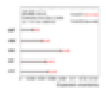
\includegraphics[width=0.48\textwidth]{\main/section2/plots/comb/ATLAS_5XS.pdf}%
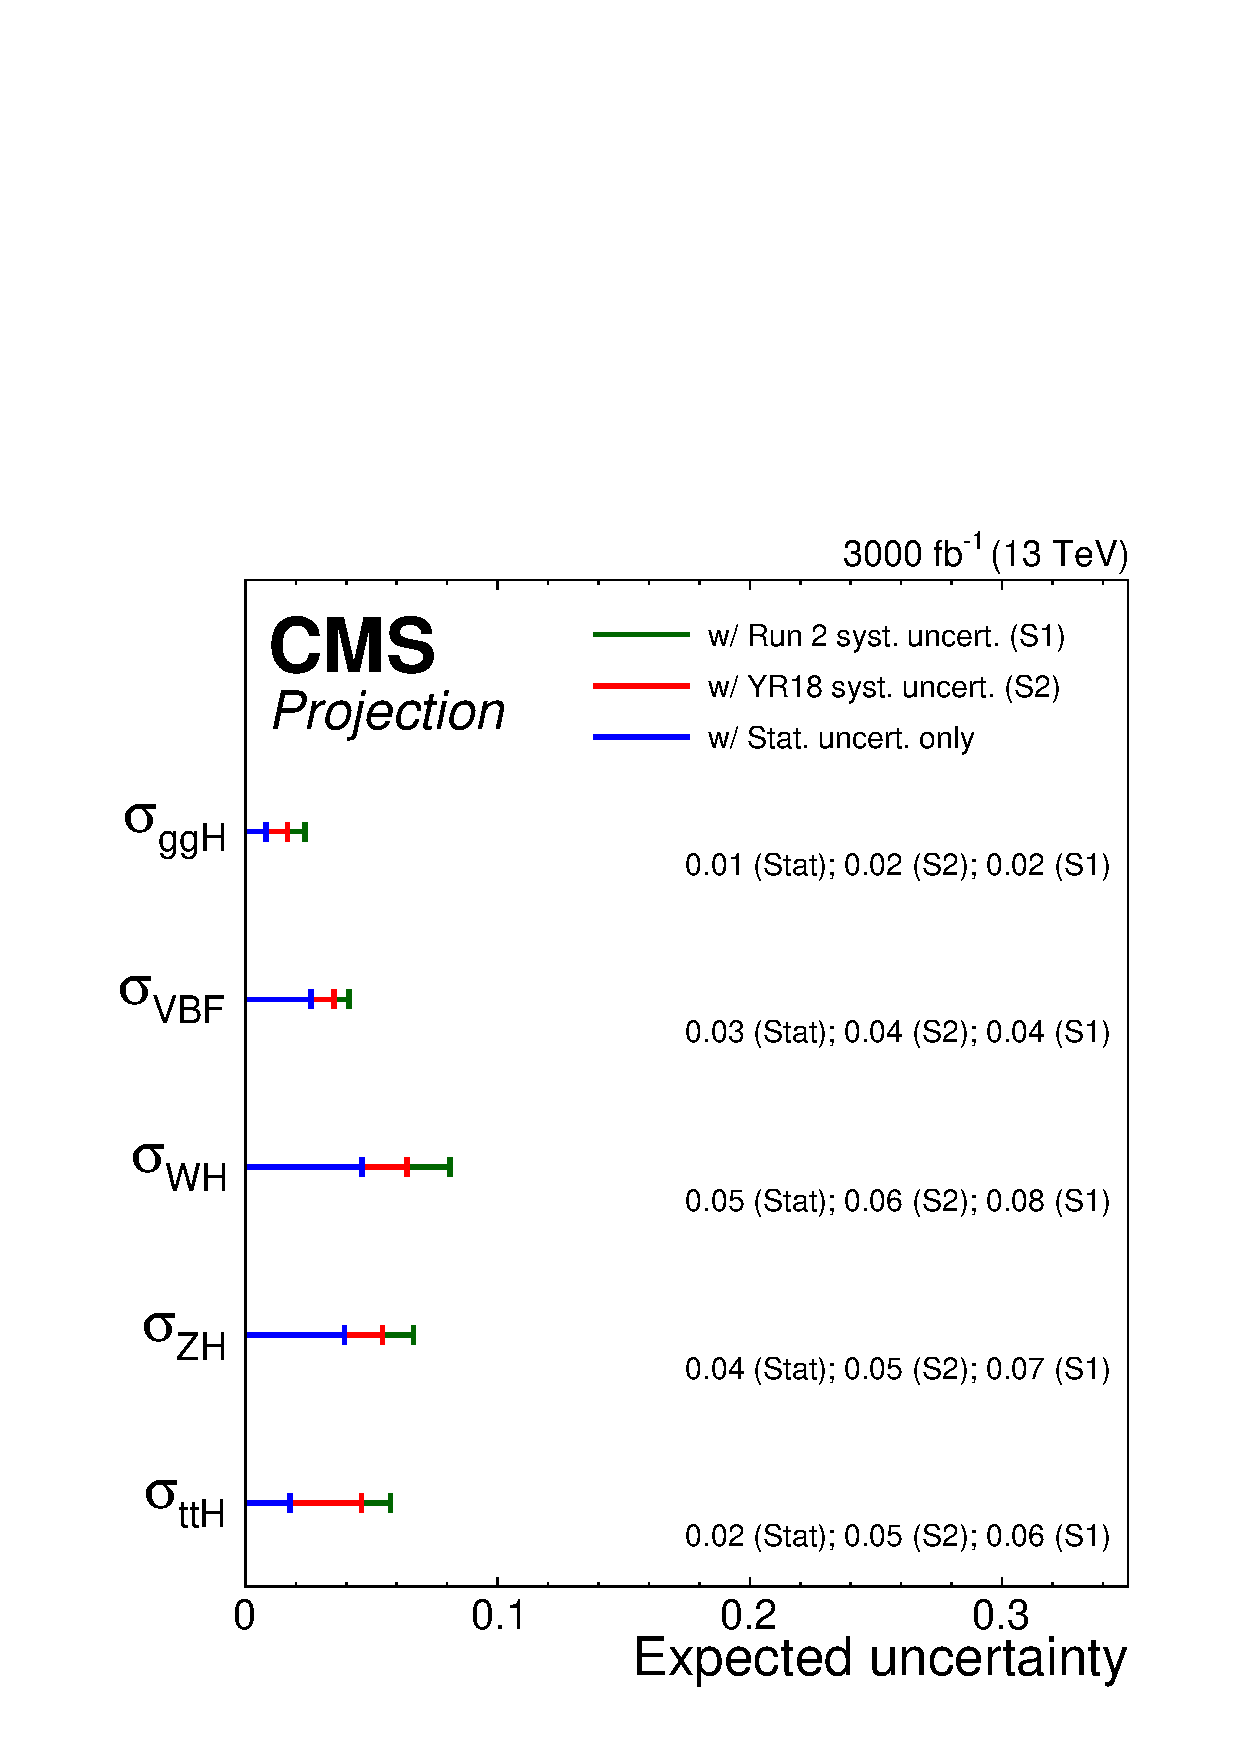
\includegraphics[width=0.48\textwidth]{\main/section2/plots/comb/summary_noinc_A1_5P_3000.pdf}%
\caption{Summary plot showing the total expected $\pm 1\sigma$ uncertainties in S1 (with Run~2 systematic uncertainties~\cite{Sirunyan:2018koj}) and S2 (with YR18 systematic uncertainties) on the per-production-mode cross sections normalized to the SM predictions  for  ATLAS (left) and CMS (right). The statistical-only component of the uncertainty is also shown.\wip{add ATLAS results, update all with xsec}}
\label{fig:summary_A1_5P}
\end{figure}


\begin{table}[hbtp]
\centering
\caption{The expected $\pm 1\sigma$ uncertainties, expressed as percentages, on the per-production-mode cross sections normalized to the SM values  for  ATLAS (left) and CMS (right). Values are given for both S1 (with Run~2 systematic uncertainties~\cite{Sirunyan:2018koj}) and S2 (with YR18 systematic uncertainties). The total uncertainty is decomposed into four components: statistical (Stat), signal theory (SigTh), background theory (BkgTh) and experimental (Exp).\wip{add ATLAS results, update all with xsec}}
\begin{tabular}{@{} l c c@{\hskip 0.15in} c c c c @{}}
 \hline
  &  & \multicolumn{5}{c}{3000 $\text{fb}^{-1}$ uncertainty [\%]} \\
  &  & Total & Stat & Exp & SigTh & BkgTh \\
 \hline
\multirow{2}{*}{$\sigma_{\mathrm{ggH}}$} & S1  & 2.4& 0.8 & 1.2 & 1.6 & 0.9  \\[1pt]
                        & S2  & 1.7& 0.8 & 0.9 & 0.9 & 0.6  \\[4pt]
\multirow{2}{*}{$\sigma_{\mathrm{VBF}}$} & S1  & 4.1& 2.6 & 2.1 & 2.0 & 1.3  \\[1pt]
                        & S2  & 3.5& 2.6 & 1.6 & 1.8 & 0.3  \\[4pt]
\multirow{2}{*}{$\sigma_{\mathrm{WH}}$} & S1  & 8.1& 4.6 & 5.2 & 2.6 & 3.3  \\[1pt]
                        & S2  & 6.4& 4.6 & 3.2 & 1.5 & 2.7  \\[4pt]
\multirow{2}{*}{$\sigma_{\mathrm{ZH}}$} & S1  & 6.7& 3.9 & 2.1 & 4.3 & 2.5  \\[1pt]
                        & S2  & 5.4& 3.9 & 1.7 & 2.4 & 2.3  \\[4pt]
\multirow{2}{*}{$\sigma_{\mathrm{ttH}}$} & S1  & 5.8& 1.8 & 3.1 & 1.9 & 4.1  \\[1pt]
                        & S2  & 4.6& 1.8 & 2.4 & 1.1 & 3.4  \\[4pt]
\hline
\end{tabular}
\begin{tabular}{@{} l c c@{\hskip 0.15in} c c c c @{}}
 \hline
  &  & \multicolumn{5}{c}{3000 $\text{fb}^{-1}$ uncertainty [\%]} \\
  &  & Total & Stat & Exp & SigTh & BkgTh \\
 \hline
\multirow{2}{*}{$\sigma_{\mathrm{ggH}}$} & S1  & 2.4& 0.8 & 1.2 & 1.6 & 0.9  \\[1pt]
                        & S2  & 1.7& 0.8 & 0.9 & 0.9 & 0.6  \\[4pt]
\multirow{2}{*}{$\sigma_{\mathrm{VBF}}$} & S1  & 4.1& 2.6 & 2.1 & 2.0 & 1.3  \\[1pt]
                        & S2  & 3.5& 2.6 & 1.6 & 1.8 & 0.3  \\[4pt]
\multirow{2}{*}{$\sigma_{\mathrm{WH}}$} & S1  & 8.1& 4.6 & 5.2 & 2.6 & 3.3  \\[1pt]
                        & S2  & 6.4& 4.6 & 3.2 & 1.5 & 2.7  \\[4pt]
\multirow{2}{*}{$\sigma_{\mathrm{ZH}}$} & S1  & 6.7& 3.9 & 2.1 & 4.3 & 2.5  \\[1pt]
                        & S2  & 5.4& 3.9 & 1.7 & 2.4 & 2.3  \\[4pt]
\multirow{2}{*}{$\sigma_{\mathrm{ttH}}$} & S1  & 5.8& 1.8 & 3.1 & 1.9 & 4.1  \\[1pt]
                        & S2  & 4.6& 1.8 & 2.4 & 1.1 & 3.4  \\[4pt]
\hline
\end{tabular}
\label{tab:summary_A1_5P}
\vspace{0.5cm}
\end{table}

Figure~\ref{fig:corr_A1_5P} shows the correlation coefficients between the production cross sections  parameters in S2. The correlations in this case are small compared to the per-decay measurements since production modes are generally well-isolated by independent analysis categories and the main theoretical uncertainties on the SM signal expectation are uncorrelated.

\begin{figure}[hbtp]
\centering
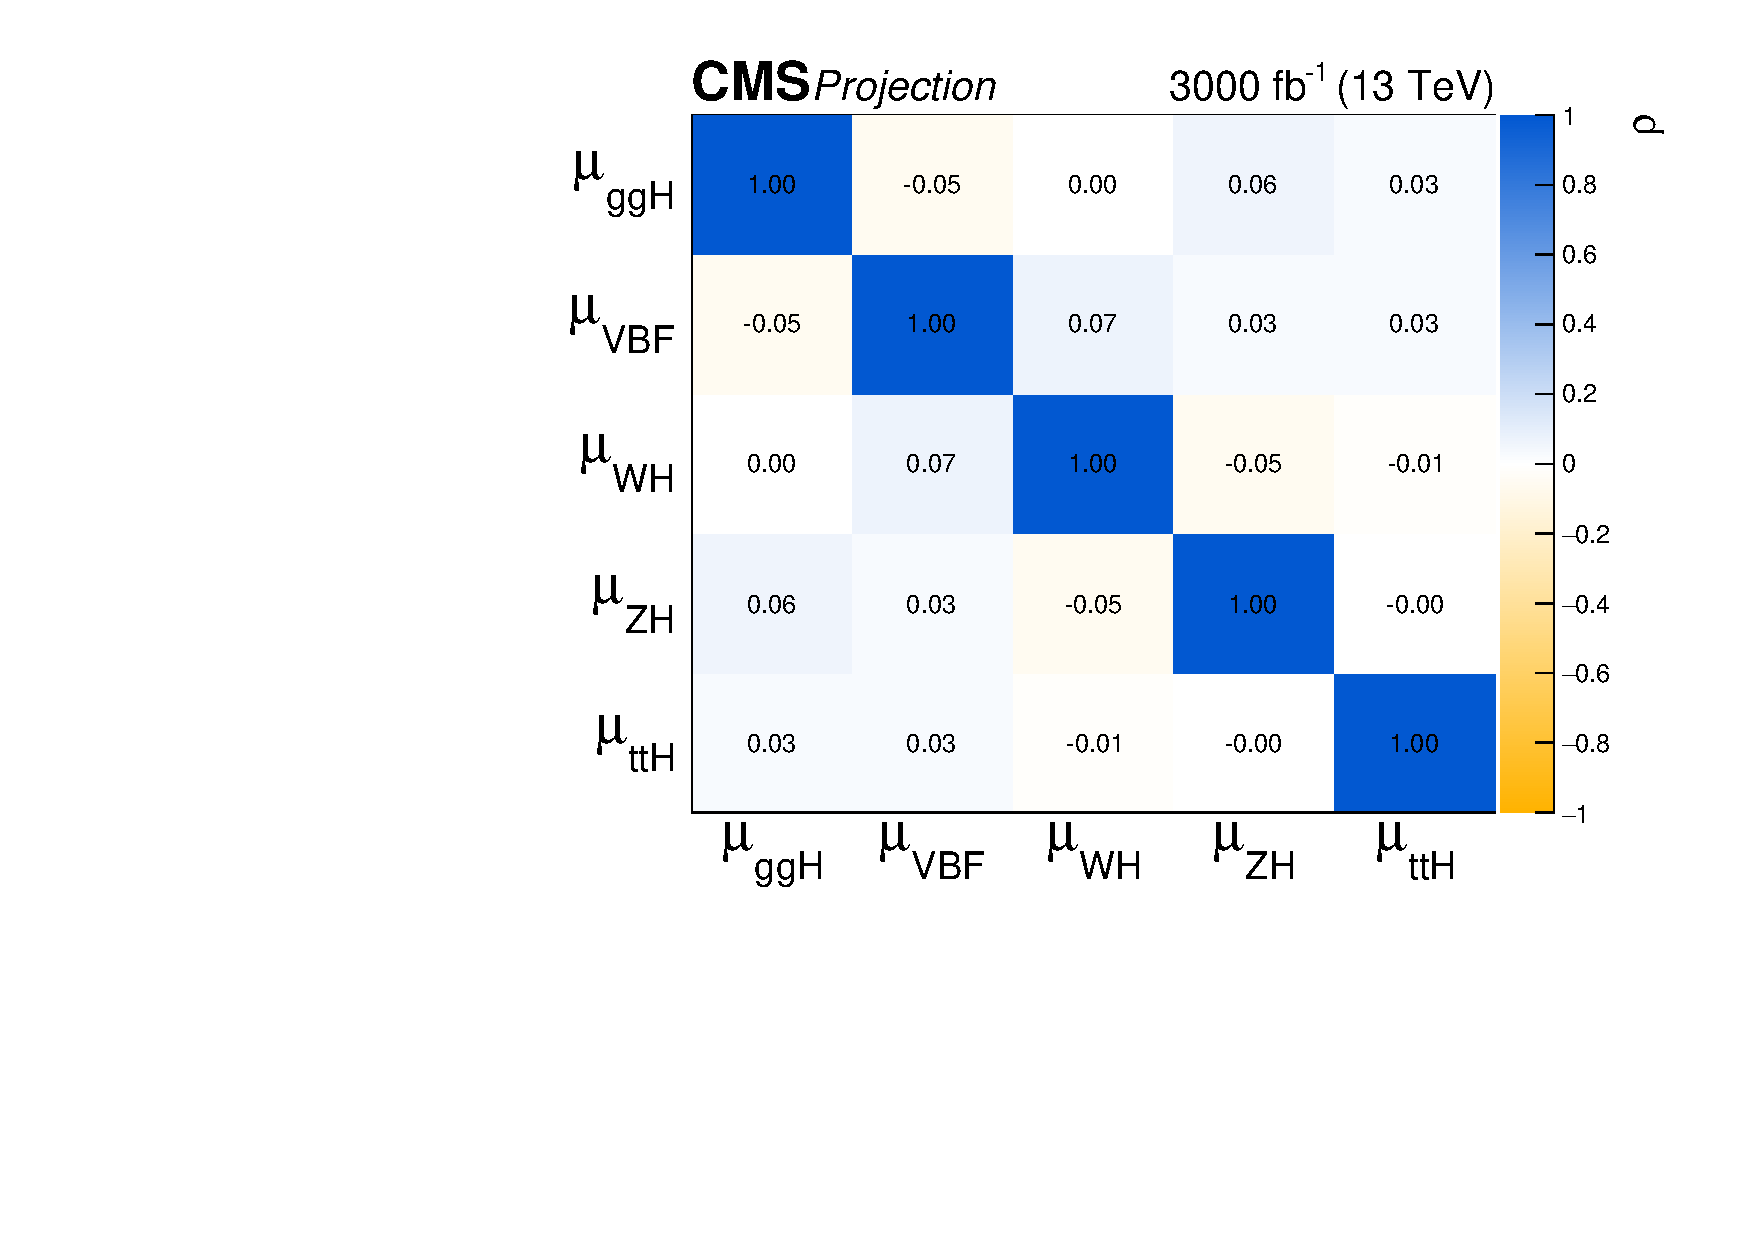
\includegraphics[width=0.48\textwidth]{\main/section2/plots/comb/correlations_A1_5P_S2_3000.pdf}%
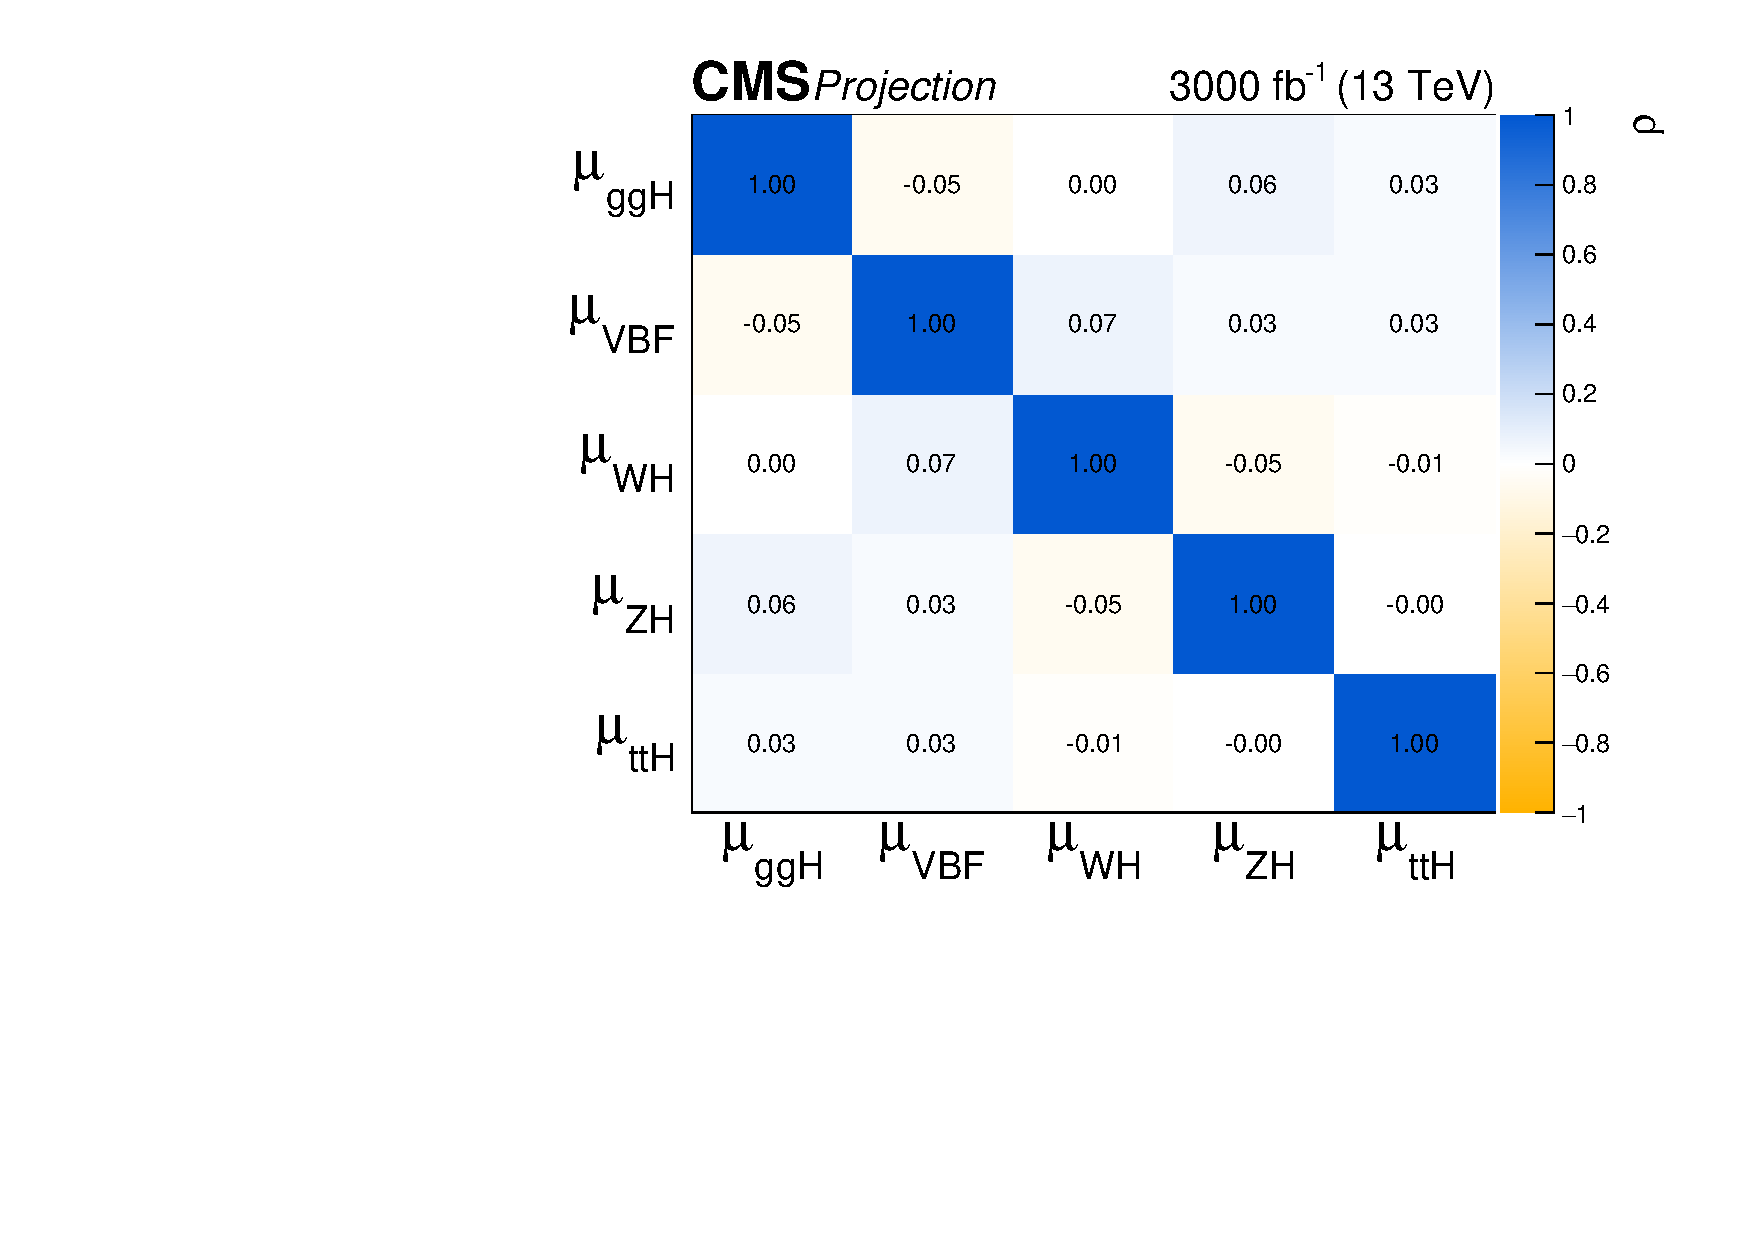
\includegraphics[width=0.48\textwidth]{\main/section2/plots/comb/correlations_A1_5P_S2_3000.pdf}%
\caption{Correlation coefficients ($\rho$) between the per-production-mode cross sections for S2 (with YR18 systematic uncertainties) for  ATLAS (left) and CMS (right). \wip{add ATLAS results, update all with xsec}}
\label{fig:corr_A1_5P}
\end{figure}

Figure~\ref{fig:comb_5P} shows the expected $\pm 1\sigma$ uncertainties for the combined ATLAS-CMS projections of the production modes cross sections for S2. 

\begin{figure}[hbtp]
\centering
%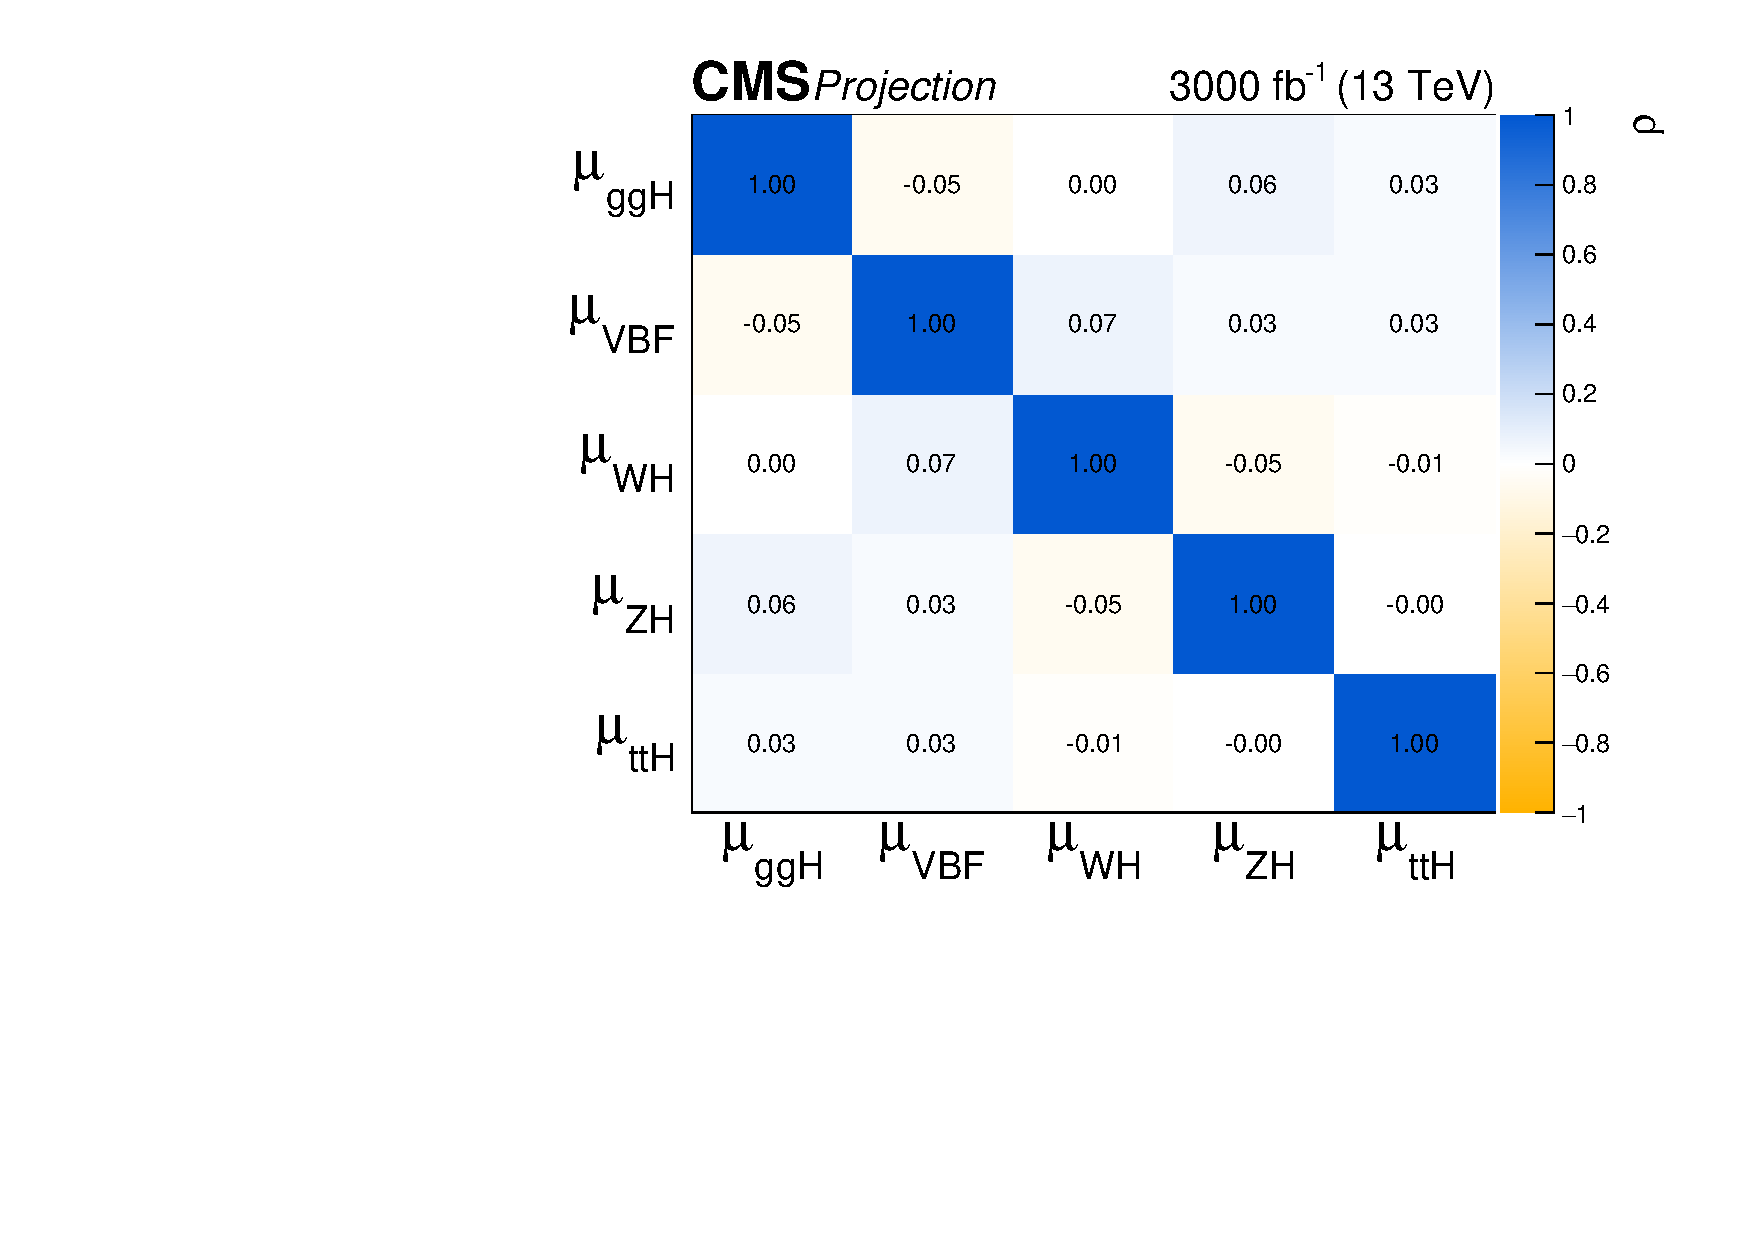
\includegraphics[width=0.48\textwidth]{\main/section2/plots/comb/correlations_A1_5P_S2_3000.pdf}%
\caption{Summary plot showing the total expected $\pm 1\sigma$ uncertainties in S2  (with YR18 systematic uncertainties) on the per-production-mode cross sections normalized to the SM predictions combining  ATLAS and CMS.}
\label{fig:comb_5P}
\end{figure}

%-----------------------------------------------------

\subsubsection{Signal strength per-decay mode}

The expected $\pm 1\sigma$ uncertainties on the per-decay-mode signal strength parameters in S1 and S2 are summarised in Figure~\ref{fig:summary_A1_5D} with numerical values given in Table~\ref{tab:summary_A1_5D}. The table additionally gives the breakdown of the uncertainty into four components: statistical, signal theory, background theory and experimental. The S2 uncertainties range from $3$--$4\%$, with the exception of that on $\mu^{\mu\mu}$ at $10\%$. The S1 uncertainties are up to a factor of 1.5 larger than those in S2, reflecting the larger systematic component. The dominant uncertainty contribution is found to vary with the scenario and the integrated luminosity of the projection. The systematic uncertainties generally dominate in both S1 and S2. In S2 the signal theory uncertainty is the largest, or joint-largest, component for all parameters except $\mu^{\mu\mu}$, which remains limited by statistics due to the small $\hmm$ branching fraction. The $\mu^{\mu\mu}$ uncertainty using the Run~2 dimuon mass resolution instead of the Phase-2 expectation is $14\%$.


\begin{figure}[hbtp]
\centering
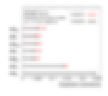
\includegraphics[width=0.48\textwidth]{\main/section2/plots/comb/ATLAS_5BR.pdf}%
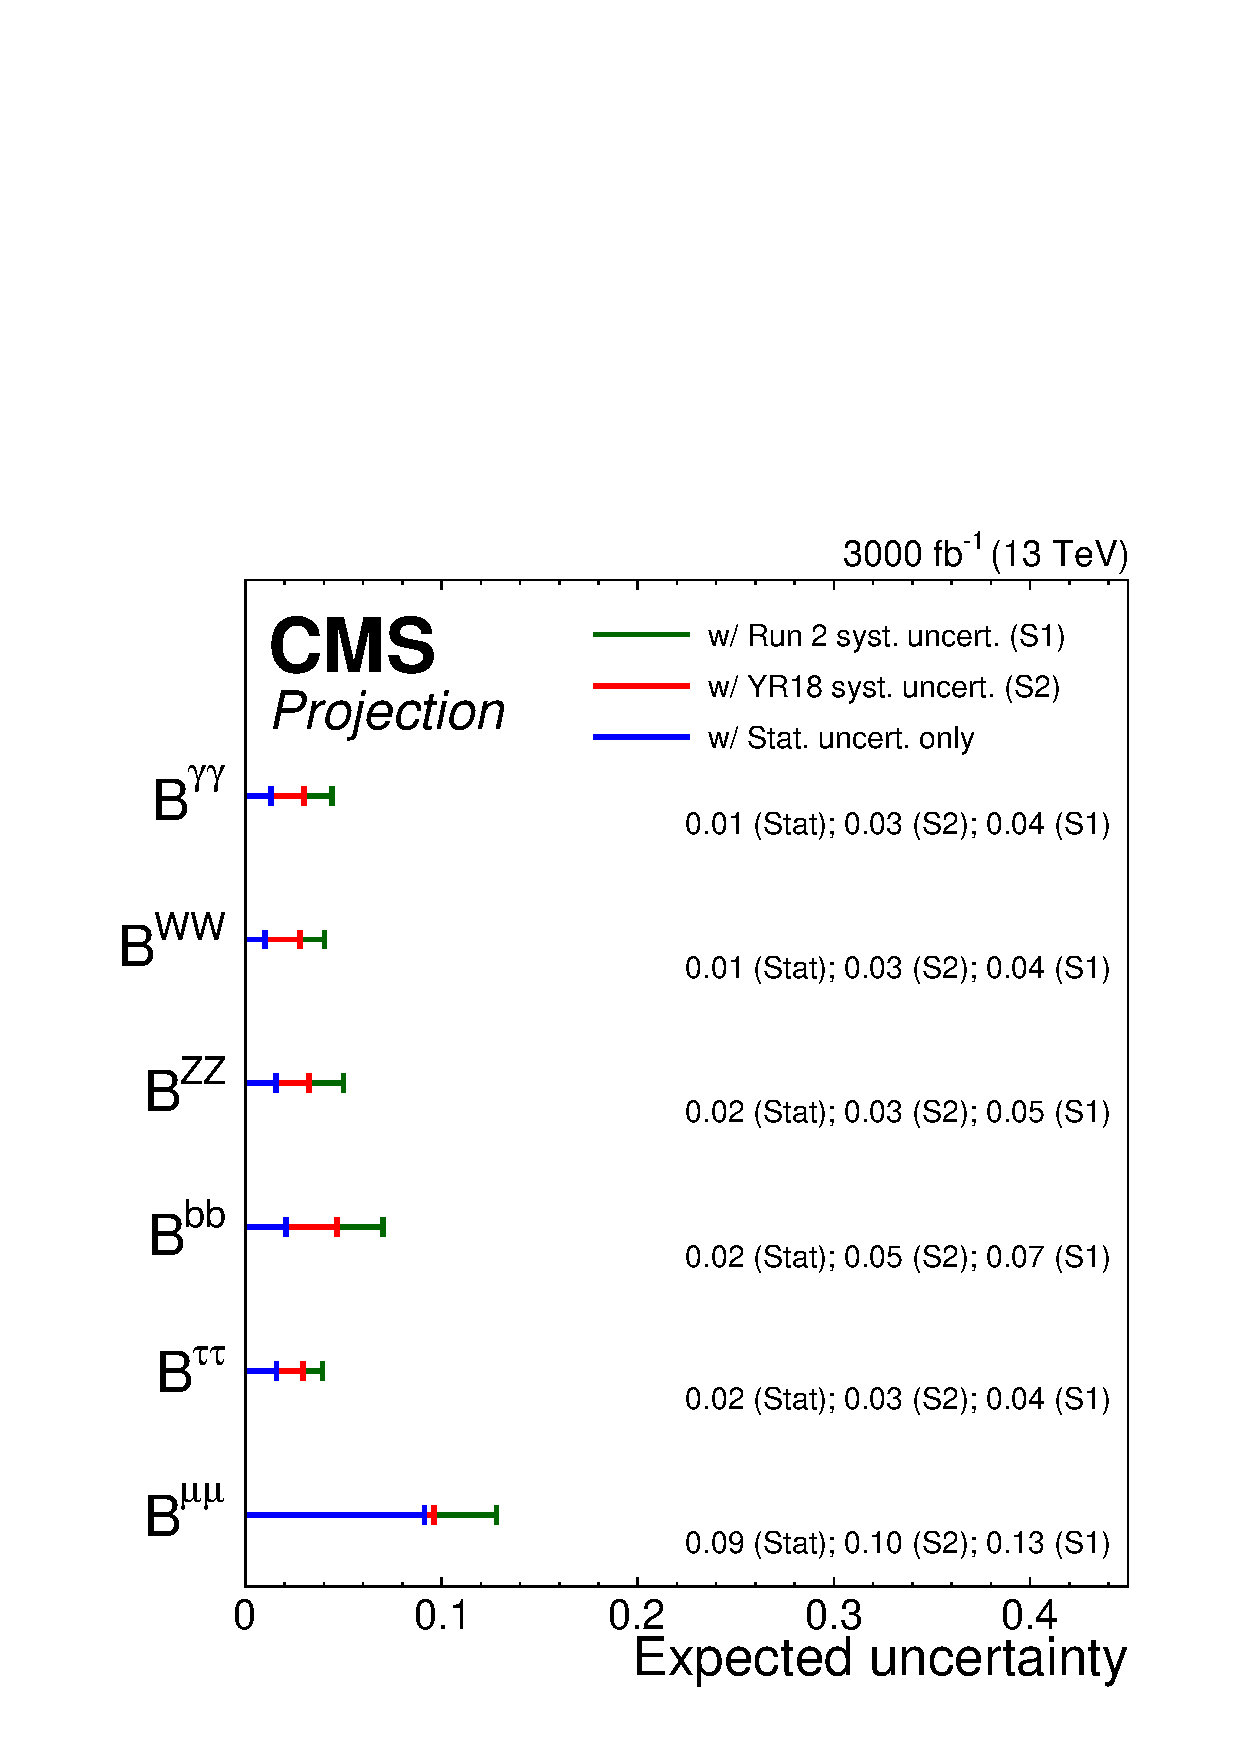
\includegraphics[width=0.48\textwidth]{\main/section2/plots/comb/summary_noinc_A1_5D_3000.pdf}%
\caption{Summary plot showing the total expected $\pm 1\sigma$ uncertainties in S1 (with Run~2 systematic uncertainties~\cite{Sirunyan:2018koj}) and S2 (with YR18 systematic uncertainties) on the branching ratios normalized to the SM expectations for ATLAS (left) and CMS (right). The statistical-only component of the uncertainty is also shown.\wip{add ATLAS results, update all with Br}}
\label{fig:summary_A1_5D}
\end{figure}


\begin{table}[hbtp]
\centering
\caption{The expected $\pm 1\sigma$ uncertainties, expressed as percentages, on the Higgs boson branching ratios normalized by the SM expectations for ATLAS (left) and CMS (right). Values are given for both S1 (with Run~2 systematic uncertainties~\cite{Sirunyan:2018koj}) and S2 (with YR18 systematic uncertainties). The total uncertainty is decomposed into four components: statistical (Stat), signal theory (SigTh), background theory (BkgTh) and experimental (Exp).\wip{add ATLAS results, update all with Br}}
\begin{tabular}{@{} l c c@{\hskip 0.15in} c c c c @{}}
 \hline
  &  & \multicolumn{5}{c}{3000 $\text{fb}^{-1}$ uncertainty [\%]} \\
  &  & Total & Stat & Exp & SigTh & BkgTh \\
 \hline
\multirow{2}{*}{$\mathrm{B}^{\gamma\gamma}$} & S1  & 4.4& 1.3 & 2.6 & 3.3 & 0.3  \\[1pt]
                        & S2  & 3.0& 1.3 & 1.7 & 1.9 & 0.3  \\[4pt]
\multirow{2}{*}{$\mathrm{B}^{\mathrm{WW}}$} & S1  & 4.0& 1.0 & 1.4 & 3.5 & 1.0  \\[1pt]
                        & S2  & 2.8& 1.0 & 1.1 & 2.2 & 0.9  \\[4pt]
\multirow{2}{*}{$\mathrm{B}^{\mathrm{ZZ}}$} & S1  & 5.0& 1.6 & 2.5 & 3.5 & 1.9  \\[1pt]
                        & S2  & 3.2& 1.6 & 1.7 & 2.1 & 0.7  \\[4pt]
\multirow{2}{*}{$\mathrm{B}^{\mathrm{bb}}$} & S1  & 7.0& 2.1 & 2.3 & 5.2 & 3.6  \\[1pt]
                        & S2  & 4.7& 2.1 & 1.7 & 2.4 & 2.9  \\[4pt]
\multirow{2}{*}{$\mathrm{B}^{\tau\tau }$} & S1  & 3.9& 1.6 & 1.9 & 2.6 & 1.5  \\[1pt]
                        & S2  & 2.9& 1.6 & 1.4 & 1.9 & 0.6  \\[4pt]
\multirow{2}{*}{$\mathrm{B}^{\mu\mu}$} & S1  & 12.8& 9.1 & 7.6 & 4.7 & 0.8  \\[1pt]
                        & S2  & 9.6& 9.1 & 1.7 & 2.6 & 0.8  \\[4pt]
\hline
\end{tabular}
\begin{tabular}{@{} l c c@{\hskip 0.15in} c c c c @{}}
 \hline
  &  & \multicolumn{5}{c}{3000 $\text{fb}^{-1}$ uncertainty [\%]} \\
  &  & Total & Stat & Exp & SigTh & BkgTh \\
 \hline
\multirow{2}{*}{$\mathrm{B}^{\gamma\gamma}$} & S1  & 4.4& 1.3 & 2.6 & 3.3 & 0.3  \\[1pt]
                        & S2  & 3.0& 1.3 & 1.7 & 1.9 & 0.3  \\[4pt]
\multirow{2}{*}{$\mathrm{B}^{\mathrm{WW}}$} & S1  & 4.0& 1.0 & 1.4 & 3.5 & 1.0  \\[1pt]
                        & S2  & 2.8& 1.0 & 1.1 & 2.2 & 0.9  \\[4pt]
\multirow{2}{*}{$\mathrm{B}^{\mathrm{ZZ}}$} & S1  & 5.0& 1.6 & 2.5 & 3.5 & 1.9  \\[1pt]
                        & S2  & 3.2& 1.6 & 1.7 & 2.1 & 0.7  \\[4pt]
\multirow{2}{*}{$\mathrm{B}^{\mathrm{bb}}$} & S1  & 7.0& 2.1 & 2.3 & 5.2 & 3.6  \\[1pt]
                        & S2  & 4.7& 2.1 & 1.7 & 2.4 & 2.9  \\[4pt]
\multirow{2}{*}{$\mathrm{B}^{\tau\tau }$} & S1  & 3.9& 1.6 & 1.9 & 2.6 & 1.5  \\[1pt]
                        & S2  & 2.9& 1.6 & 1.4 & 1.9 & 0.6  \\[4pt]
\multirow{2}{*}{$\mathrm{B}^{\mu\mu}$} & S1  & 12.8& 9.1 & 7.6 & 4.7 & 0.8  \\[1pt]
                        & S2  & 9.6& 9.1 & 1.7 & 2.6 & 0.8  \\[4pt]
\hline
\end{tabular}
\label{tab:summary_A1_5D}
\vspace{0.5cm}
\end{table}

Another important aspect of the projected measurements is how the correlations between the measured parameters are expected to evolve. Correlations arise when analysis channels are sensitive to more than one production or decay mode and the chosen fit observables do not fully distinguish between these. In addition, correlations may arise when the same systematic uncertainties apply to multiple production or decay modes. Figure~\ref{fig:corr_A1_5D} shows the correlation coefficients between the signal strength parameters in S2. The correlations range up to $+0.44$, and are largest between modes where the sensitivity is dominated by gluon-fusion production. This reflects the impact of the theory uncertainties affecting the SM prediction of the gluon-fusion production rate.

\begin{figure}[hbtp]
\centering
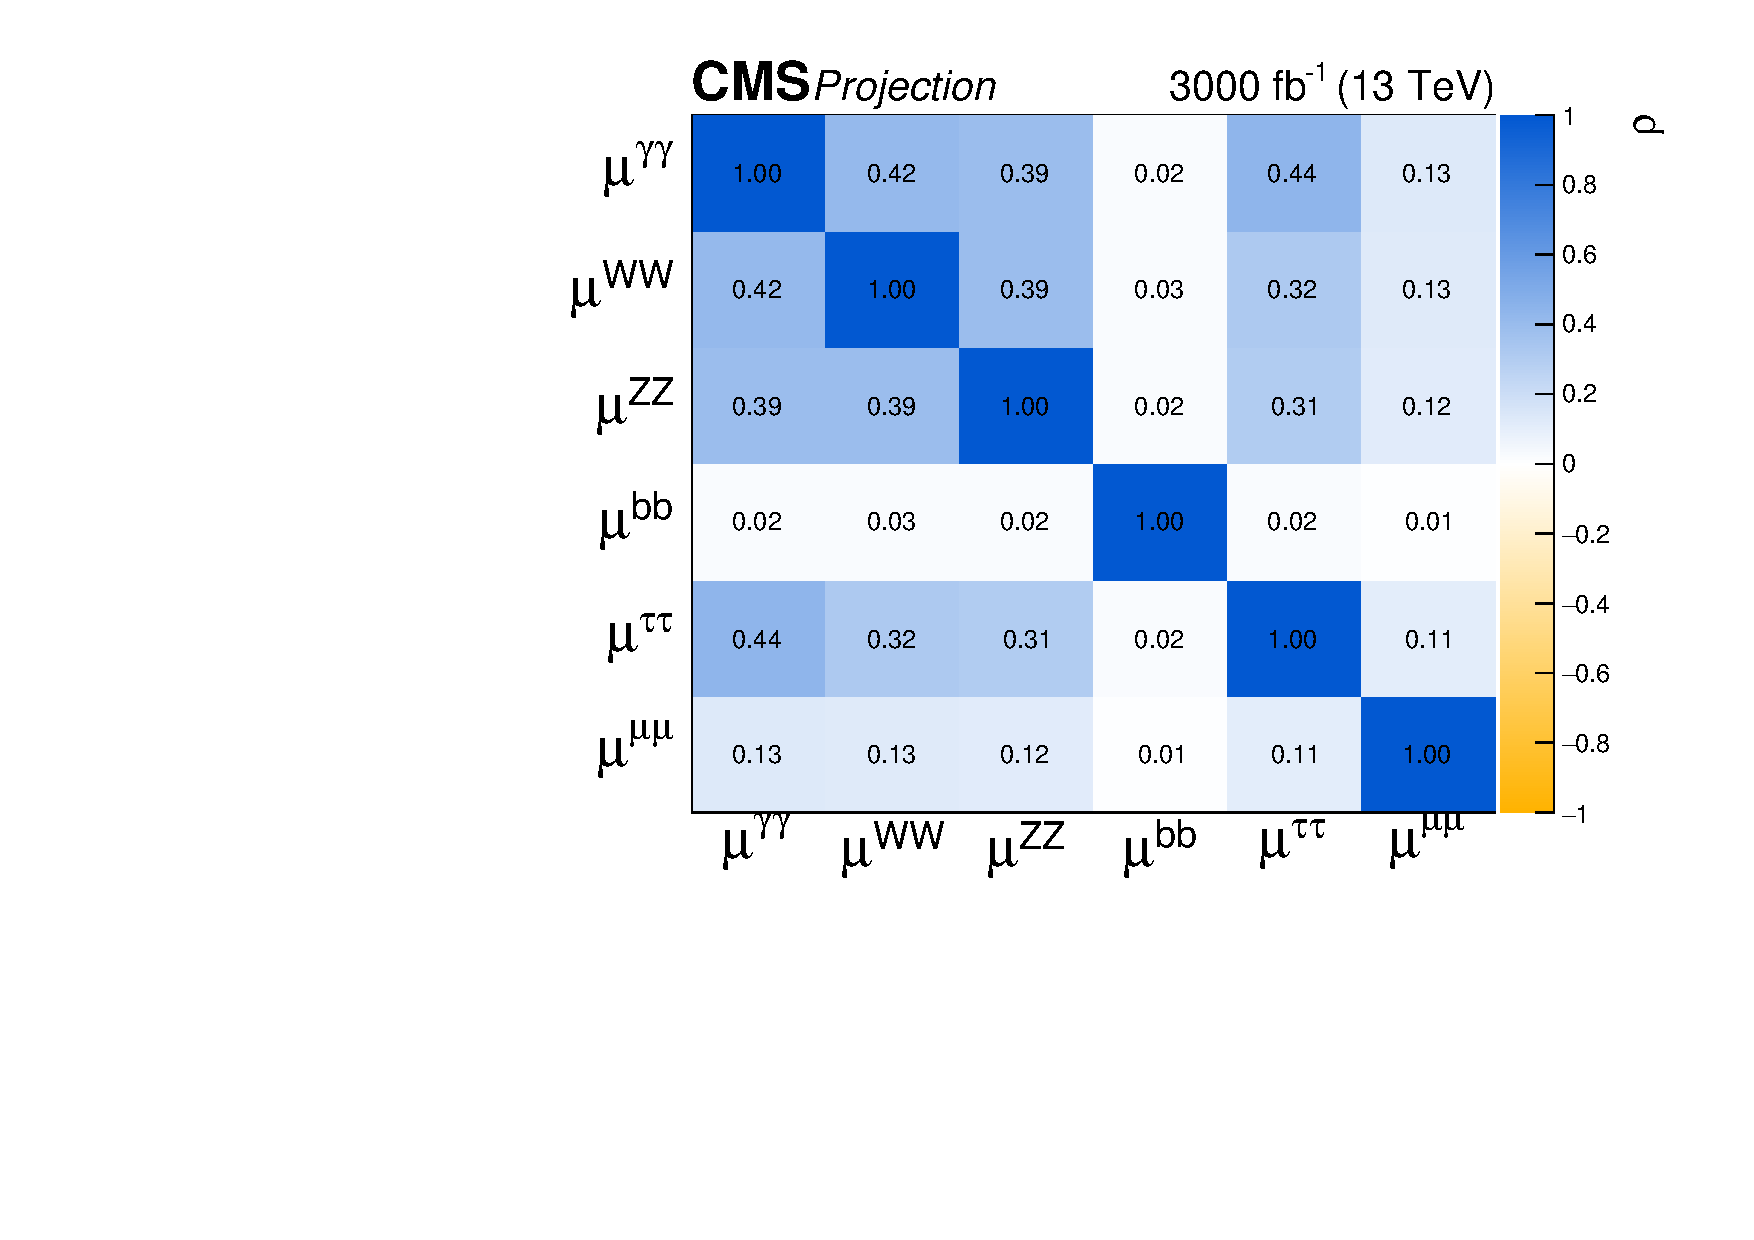
\includegraphics[width=0.48\textwidth]{\main/section2/plots/comb/correlations_A1_5D_S2_3000.pdf}%
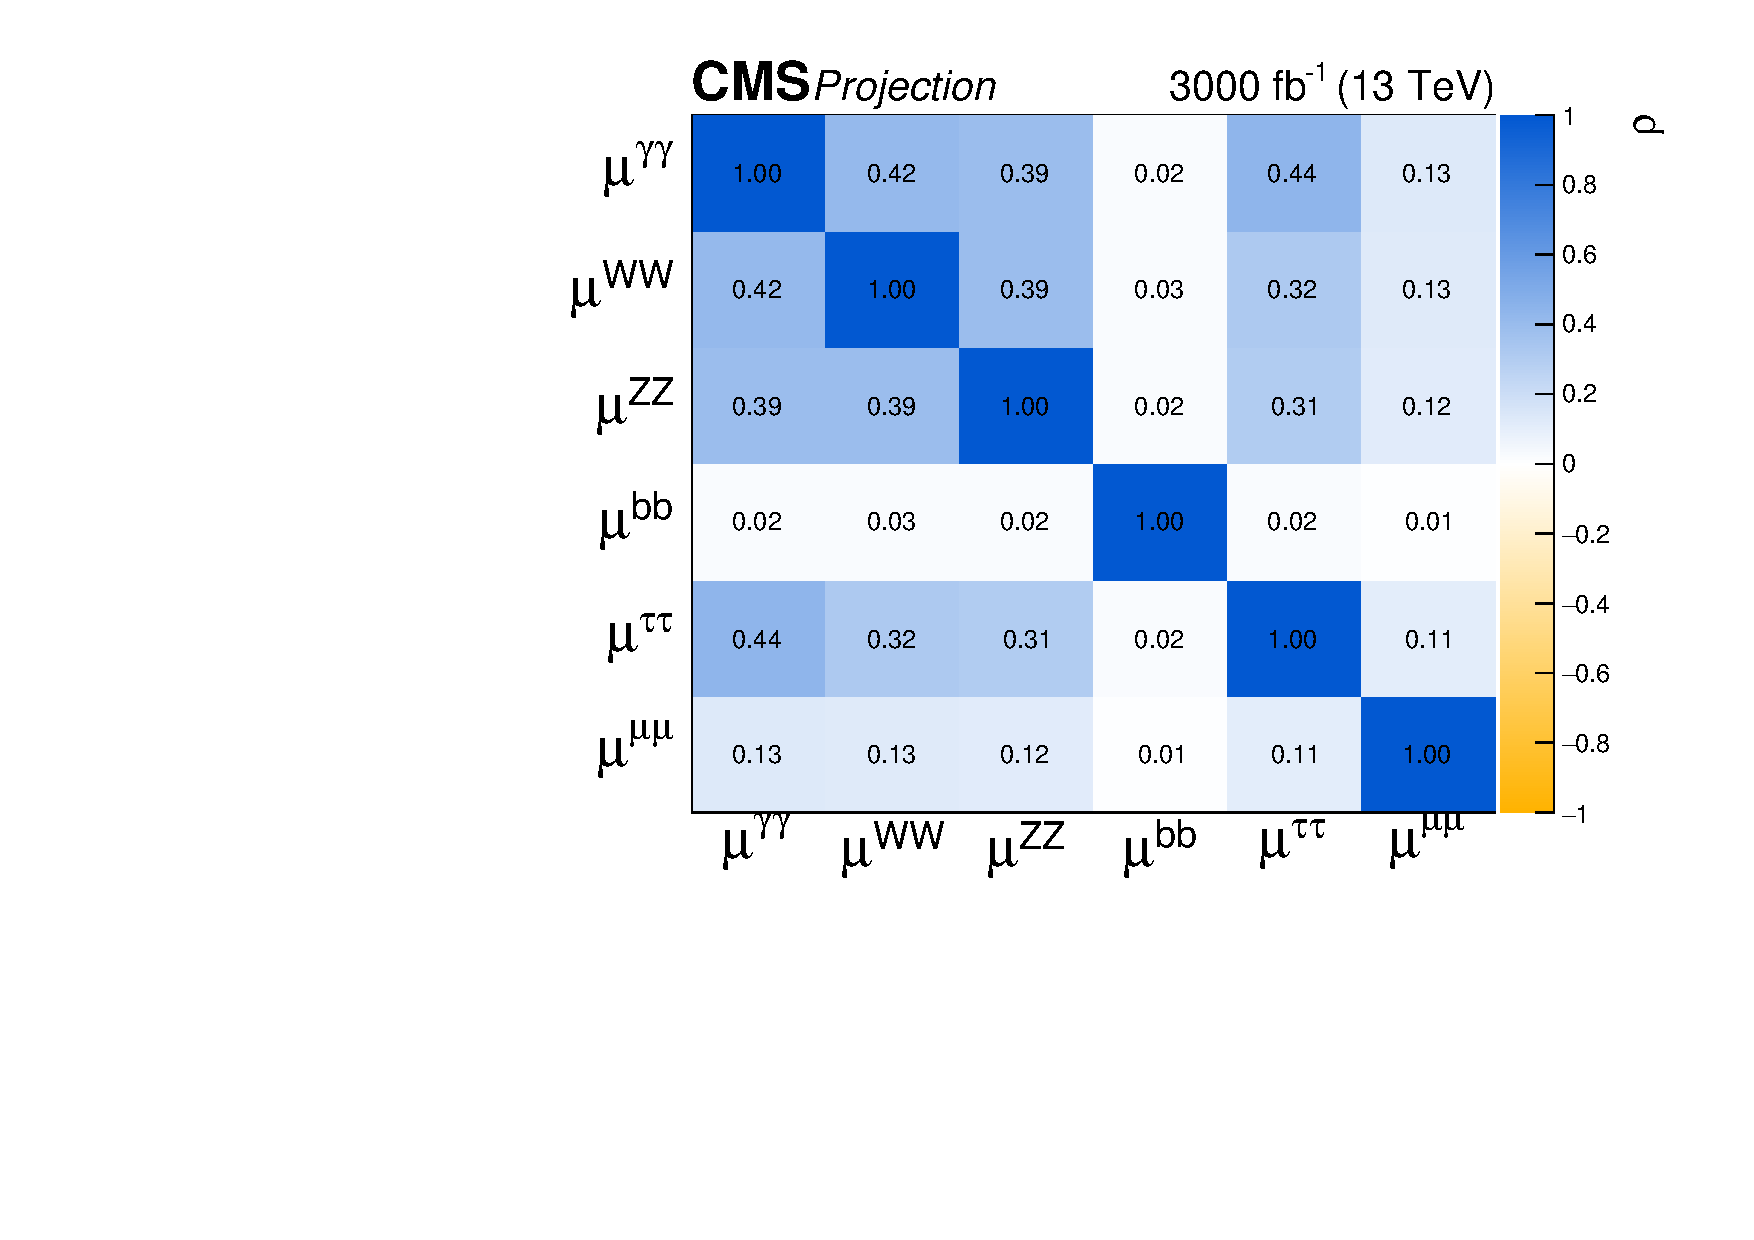
\includegraphics[width=0.48\textwidth]{\main/section2/plots/comb/correlations_A1_5D_S2_3000.pdf}%
\caption{Correlation coefficients ($\rho$) between the different Higgs boson branching ratios normalized to the SM values for S2 (with YR18 systematic uncertainties) for ATLAS (left) and CMS (right).\wip{add ATLAS results, move to BR}}
\label{fig:comb_5D}
\end{figure}

Figure~\ref{fig:br_comb} shows the expected $\pm 1\sigma$ uncertainties for the combined ATLAS-CMS projections of the Higgs boson branching fractions normalized to the corresponding SM values for S2.

\begin{figure}[hbtp]
\centering
%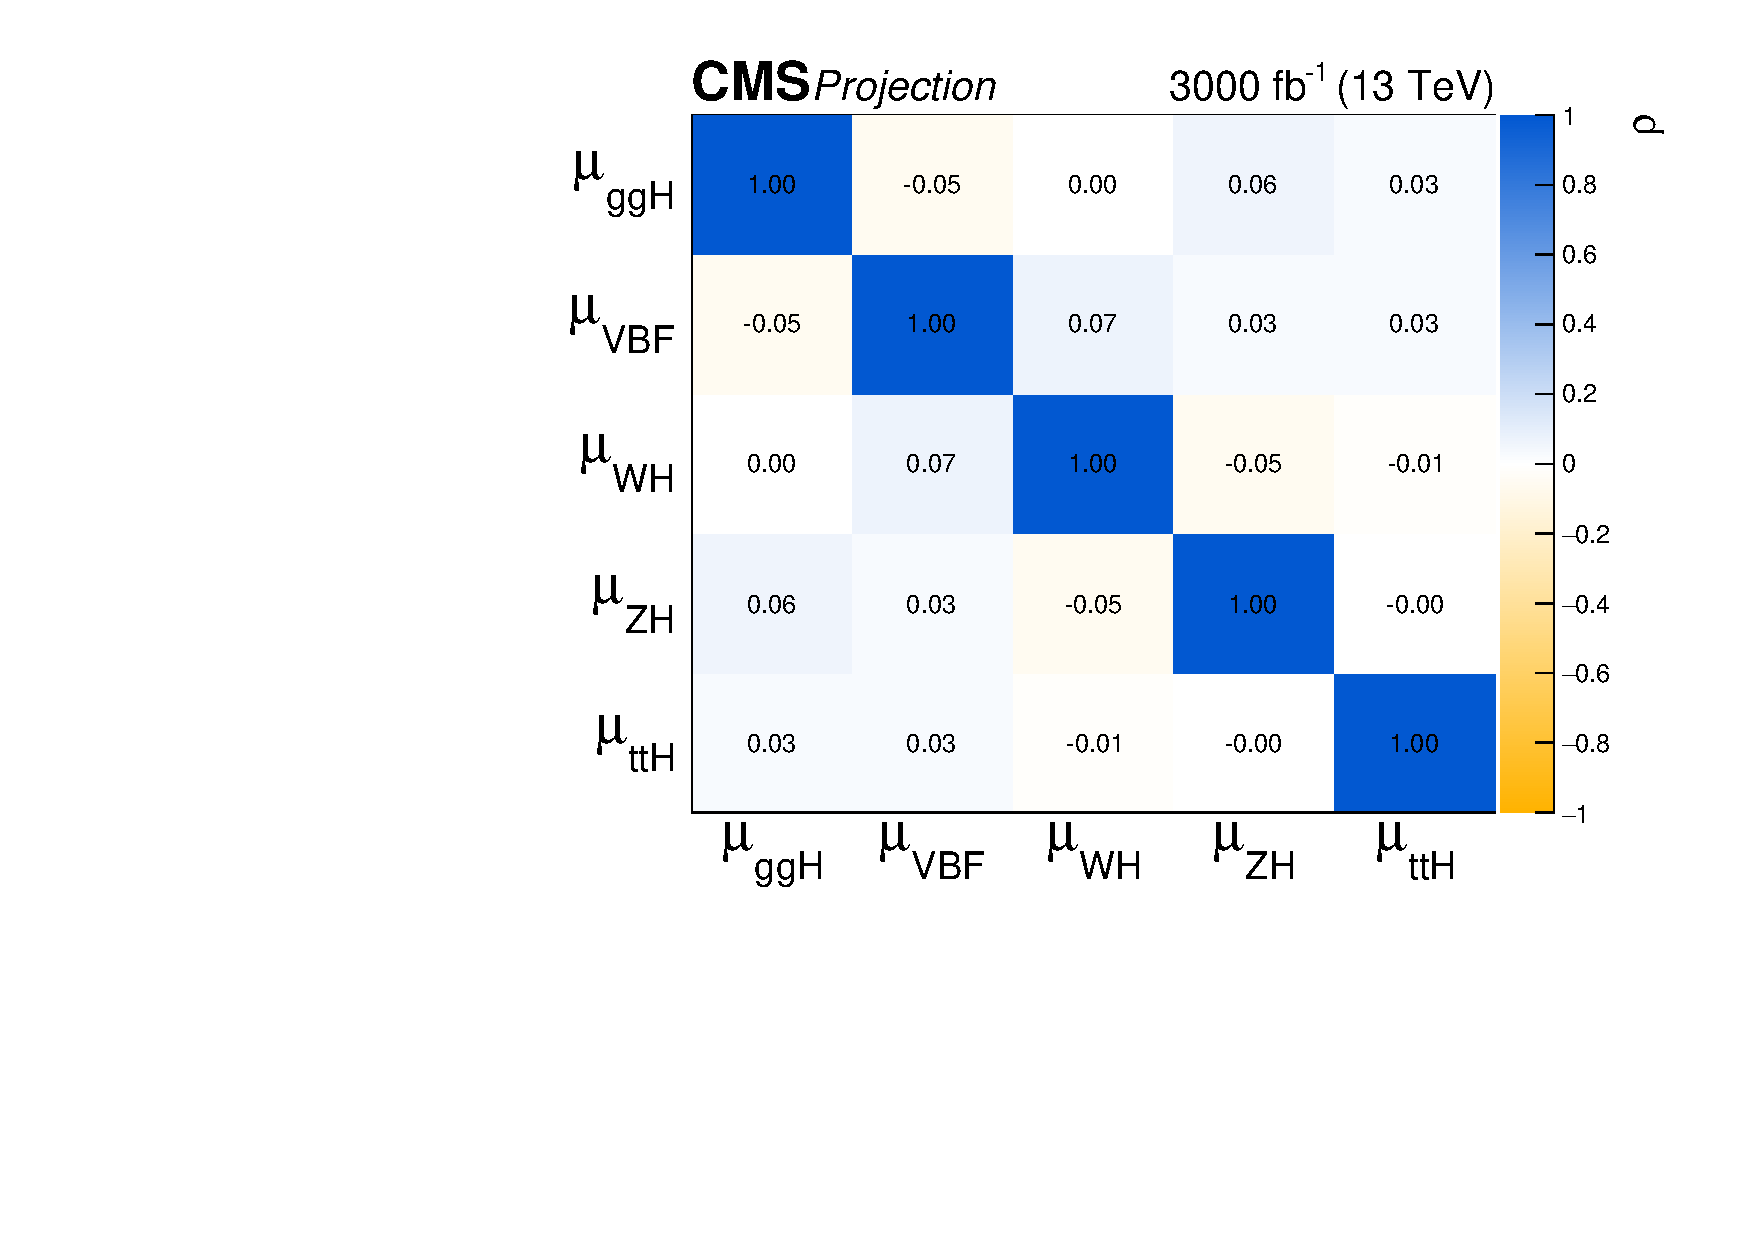
\includegraphics[width=0.48\textwidth]{\main/section2/plots/comb/correlations_A1_5P_S2_3000.pdf}%
\caption{Summary plot showing the total expected $\pm 1\sigma$ uncertainties in S2  (with YR18 systematic uncertainties) on the Higgs boson branching fractions normalized to the SM predictions combining  ATLAS and CMS.}
\label{fig:br_comb}
\end{figure}



\subsubsection{Production mode cross-sections in different decay channels}
The expected $\pm 1\sigma$ uncertainties on the production mode cross sections in the different decay channels in S1 and S2 are summarised in Figure~\ref{fig:summary_A1_5PD} with numerical values given in Table~\ref{tab:summary_A1_5PD}. The table additionally gives the breakdown of the uncertainty into four components: statistical, signal theory, background theory and experimental. 


\begin{figure}[hbtp]
\centering
\includegraphics[width=0.48\textwidth]{\main/section2/plots/comb/summary_A1_5PD_3000.pdf}%
\includegraphics[width=0.48\textwidth]{\main/section2/plots/comb/summary_A1_5PD_3000.pdf}%
\caption{Summary plot showing the total expected $\pm 1\sigma$ uncertainties in S1 (with Run~2 systematic uncertainties~\cite{Sirunyan:2018koj}) and S2 (with YR18 systematic uncertainties) on the production cross sections in the different decay modes  for ATLAS (left) and CMS (right). The statistical-only component of the uncertainty is also shown.\wip{add ATLAS and CMS results}}
\label{fig:summary_A1_5PD}
\end{figure}


\begin{table}[hbtp]
\centering
\caption{The expected $\pm 1\sigma$ uncertainties, expressed as percentages, on the per-production-mode cross sections in the different decay modes  for ATLAS (left) and CMS (right). Values are given for both S1 (with Run~2 systematic uncertainties~\cite{Sirunyan:2018koj}) and S2 (with YR18 systematic uncertainties). The total uncertainty is decomposed into four components: statistical (Stat), signal theory (SigTh), background theory (BkgTh) and experimental (Exp).\wip{add ATLAS results, update all with xsec}}
\scriptsize	
\begin{tabular}{@{} l c c@{\hskip 0.15in} c c c c @{}}
 \hline
  &  & \multicolumn{5}{c}{3000 $\text{fb}^{-1}$ uncertainty [\%]} \\
  &  & Total & Stat & Exp & SigAcc & BkgTh \\
 \hline
\multirow{2}{*}{$\sigma_{\mathrm{ggH}}^{\gamma \gamma }$} & S1  & 3.9& 1.9 & 3.3 & 0.7 & 1.0  \\[1pt]
                        & S2  & 2.8& 1.9 & 2.1 & 0.8 & 0.9  \\[4pt]
\multirow{2}{*}{$\sigma_{\mathrm{ggH}}^{\mathrm{ZZ}}$} & S1  & 4.1& 2.1 & 2.7 & 1.2 & 1.7  \\[1pt]
                        & S2  & 3.0& 2.1 & 1.8 & 0.8 & 0.7  \\[4pt]
\multirow{2}{*}{$\sigma_{\mathrm{ggH}}^{\mathrm{WW}}$} & S1  & 3.6& 1.2 & 1.5 & 2.9 & 1.0  \\[1pt]
                        & S2  & 2.5& 1.2 & 1.2 & 1.6 & 0.9  \\[4pt]
\multirow{2}{*}{$\sigma_{\mathrm{ggH}}^{\tau \tau }$} & S1  & 5.7& 2.6 & 3.5 & 3.3 & 1.7  \\[1pt]
                        & S2  & 4.6& 2.6 & 2.9 & 2.3 & 0.7  \\[4pt]
\multirow{2}{*}{$\sigma_{\mathrm{ggH}}^{\mathrm{bb}}$} & S1  & 34.3& 20.6 & 10.0 & 23.7 & 3.2  \\[1pt]
                        & S2  & 24.7& 20.6 & 2.6 & 12.2 & 1.5  \\[4pt]
\multirow{2}{*}{$\sigma_{\mathrm{ggH}}^{\sigma \sigma }$} & S1  & 15.9& 13.4 & 8.0 & 2.6 & 1.9  \\[1pt]
                        & S2  & 13.5& 13.4 & 2.0 & 1.4 & 0.6  \\[4pt]
\multirow{2}{*}{$\sigma_{\mathrm{VBF}}^{\gamma \gamma }$} & S1  & 22.1& 5.2 & 19.9 & 7.9 & 1.3  \\[1pt]
                        & S2  & 12.7& 5.2 & 10.9 & 4.0 & 0.3  \\[4pt]
\multirow{2}{*}{$\sigma_{\mathrm{VBF}}^{\mathrm{ZZ}}$} & S1  & 15.1& 11.7 & 1.8 & 8.8 & 2.4  \\[1pt]
                        & S2  & 13.3& 11.7 & 1.3 & 5.9 & 0.8  \\[4pt]
\multirow{2}{*}{$\sigma_{\mathrm{VBF}}^{\mathrm{WW}}$} & S1  & 8.1& 6.3 & 2.0 & 4.4 & 1.8  \\[1pt]
                        & S2  & 7.2& 6.3 & 1.6 & 2.8 & 1.1  \\[4pt]
\multirow{2}{*}{$\sigma_{\mathrm{VBF}}^{\tau \tau }$} & S1  & 4.9& 3.8 & 2.0 & 2.8 & 1.5  \\[1pt]
                        & S2  & 4.2& 3.8 & 1.3 & 1.2 & 0.4  \\[4pt]
\multirow{2}{*}{$\sigma_{\mathrm{VBF}}^{\sigma \sigma }$} & S1  & 57.3& 53.2 & 11.3 & 18.0 & 4.5  \\[1pt]
                        & S2  & 54.0& 53.2 & 2.6 & 9.5 & 1.0  \\[4pt]
\multirow{2}{*}{$\sigma_{\mathrm{WH}}^{\gamma \gamma }$} & S1  & 14.3& 13.6 & 3.7 & 2.0 & 1.4  \\[1pt]
                        & S2  & 13.8& 13.6 & 1.7 & 1.5 & 0.2  \\[4pt]
\multirow{2}{*}{$\sigma_{\mathrm{WH}}^{\mathrm{ZZ}}$} & S1  & 47.9& 46.5 & 7.8 & 11.2 & 2.8  \\[1pt]
                        & S2  & 47.8& 46.5 & 3.8 & 4.0 & 0.8  \\[4pt]
\multirow{2}{*}{$\sigma_{\mathrm{WH}}^{\mathrm{WW}}$} & S1  & 15.6& 12.9 & 6.5 & 5.3 & 2.2  \\[1pt]
                        & S2  & 13.7& 12.9 & 3.1 & 2.9 & 1.5  \\[4pt]
\multirow{2}{*}{$\sigma_{\mathrm{WH}}^{\mathrm{bb}}$} & S1  & 16.0& 5.6 & 9.8 & 5.3 & 10.8  \\[1pt]
                        & S2  & 9.4& 5.6 & 5.1 & 2.2 & 5.1  \\[4pt]
\multirow{2}{*}{$\sigma_{\mathrm{ZH}}^{\gamma \gamma }$} & S1  & 23.5& 23.1 & 2.9 & 3.1 & 1.5  \\[1pt]
                        & S2  & 23.2& 23.1 & 1.2 & 2.4 & 0.4  \\[4pt]
\multirow{2}{*}{$\sigma_{\mathrm{ZH}}^{\mathrm{ZZ}}$} & S1  & 82.3& 75.7 & 16.4 & 26.3 & 7.6  \\[1pt]
                        & S2  & 78.4& 75.7 & 9.9 & 15.1 & 1.3  \\[4pt]
\multirow{2}{*}{$\sigma_{\mathrm{ZH}}^{\mathrm{WW}}$} & S1  & 18.5& 17.2 & 3.5 & 5.3 & 2.4  \\[1pt]
                        & S2  & 17.7& 17.2 & 3.0 & 2.8 & 1.7  \\[4pt]
\multirow{2}{*}{$\sigma_{\mathrm{ZH}}^{\mathrm{bb}}$} & S1  & 7.9& 4.2 & 2.3 & 5.6 & 3.1  \\[1pt]
                        & S2  & 6.0& 4.2 & 1.9 & 2.9 & 2.6  \\[4pt]
\multirow{2}{*}{$\sigma_{\mathrm{ttH}}^{\gamma \gamma }$} & S1  & 9.3& 7.7 & 3.9 & 3.5 & 1.0  \\[1pt]
                        & S2  & 8.4& 7.7 & 2.7 & 1.9 & 0.2  \\[4pt]
\multirow{2}{*}{$\sigma_{\mathrm{ttH}}^{\mathrm{ZZ}}$} & S1  & 24.6& 23.6 & 4.2 & 4.9 & 2.5  \\[1pt]
                        & S2  & 24.2& 23.6 & 3.1 & 2.6 & 1.8  \\[4pt]
\multirow{2}{*}{$\sigma_{\mathrm{ttH}}^{\mathrm{WW}}$} & S1  & 11.2& 4.2 & 9.1 & 1.8 & 4.5  \\[1pt]
                        & S2  & 8.7& 4.2 & 6.9 & 1.1 & 3.0  \\[4pt]
\multirow{2}{*}{$\sigma_{\mathrm{ttH}}^{\mathrm{bb}}$} & S1  & 15.9& 2.8 & 3.9 & 0.0 & 15.2  \\[1pt]
                        & S2  & 10.8& 2.8 & 2.7 & 0.1 & 10.0  \\[4pt]
\multirow{2}{*}{$\sigma_{\mathrm{ttH}}^{\tau \tau }$} & S1  & 16.5& 8.7 & 13.1 & 3.4 & 3.5  \\[1pt]
                        & S2  & 14.2& 8.7 & 10.9 & 1.6 & 2.1  \\[4pt]
\hline
\end{tabular}\hspace{0.5cm}
\begin{tabular}{@{} l c c@{\hskip 0.15in} c c c c @{}}
 \hline
  &  & \multicolumn{5}{c}{3000 $\text{fb}^{-1}$ uncertainty [\%]} \\
  &  & Total & Stat & Exp & SigAcc & BkgTh \\
 \hline
\multirow{2}{*}{$\sigma_{\mathrm{ggH}}^{\gamma \gamma }$} & S1  & 3.9& 1.9 & 3.3 & 0.7 & 1.0  \\[1pt]
                        & S2  & 2.8& 1.9 & 2.1 & 0.8 & 0.9  \\[4pt]
\multirow{2}{*}{$\sigma_{\mathrm{ggH}}^{\mathrm{ZZ}}$} & S1  & 4.1& 2.1 & 2.7 & 1.2 & 1.7  \\[1pt]
                        & S2  & 3.0& 2.1 & 1.8 & 0.8 & 0.7  \\[4pt]
\multirow{2}{*}{$\sigma_{\mathrm{ggH}}^{\mathrm{WW}}$} & S1  & 3.6& 1.2 & 1.5 & 2.9 & 1.0  \\[1pt]
                        & S2  & 2.5& 1.2 & 1.2 & 1.6 & 0.9  \\[4pt]
\multirow{2}{*}{$\sigma_{\mathrm{ggH}}^{\tau \tau }$} & S1  & 5.7& 2.6 & 3.5 & 3.3 & 1.7  \\[1pt]
                        & S2  & 4.6& 2.6 & 2.9 & 2.3 & 0.7  \\[4pt]
\multirow{2}{*}{$\sigma_{\mathrm{ggH}}^{\mathrm{bb}}$} & S1  & 34.3& 20.6 & 10.0 & 23.7 & 3.2  \\[1pt]
                        & S2  & 24.7& 20.6 & 2.6 & 12.2 & 1.5  \\[4pt]
\multirow{2}{*}{$\sigma_{\mathrm{ggH}}^{\sigma \sigma }$} & S1  & 15.9& 13.4 & 8.0 & 2.6 & 1.9  \\[1pt]
                        & S2  & 13.5& 13.4 & 2.0 & 1.4 & 0.6  \\[4pt]
\multirow{2}{*}{$\sigma_{\mathrm{VBF}}^{\gamma \gamma }$} & S1  & 22.1& 5.2 & 19.9 & 7.9 & 1.3  \\[1pt]
                        & S2  & 12.7& 5.2 & 10.9 & 4.0 & 0.3  \\[4pt]
\multirow{2}{*}{$\sigma_{\mathrm{VBF}}^{\mathrm{ZZ}}$} & S1  & 15.1& 11.7 & 1.8 & 8.8 & 2.4  \\[1pt]
                        & S2  & 13.3& 11.7 & 1.3 & 5.9 & 0.8  \\[4pt]
\multirow{2}{*}{$\sigma_{\mathrm{VBF}}^{\mathrm{WW}}$} & S1  & 8.1& 6.3 & 2.0 & 4.4 & 1.8  \\[1pt]
                        & S2  & 7.2& 6.3 & 1.6 & 2.8 & 1.1  \\[4pt]
\multirow{2}{*}{$\sigma_{\mathrm{VBF}}^{\tau \tau }$} & S1  & 4.9& 3.8 & 2.0 & 2.8 & 1.5  \\[1pt]
                        & S2  & 4.2& 3.8 & 1.3 & 1.2 & 0.4  \\[4pt]
\multirow{2}{*}{$\sigma_{\mathrm{VBF}}^{\sigma \sigma }$} & S1  & 57.3& 53.2 & 11.3 & 18.0 & 4.5  \\[1pt]
                        & S2  & 54.0& 53.2 & 2.6 & 9.5 & 1.0  \\[4pt]
\multirow{2}{*}{$\sigma_{\mathrm{WH}}^{\gamma \gamma }$} & S1  & 14.3& 13.6 & 3.7 & 2.0 & 1.4  \\[1pt]
                        & S2  & 13.8& 13.6 & 1.7 & 1.5 & 0.2  \\[4pt]
\multirow{2}{*}{$\sigma_{\mathrm{WH}}^{\mathrm{ZZ}}$} & S1  & 47.9& 46.5 & 7.8 & 11.2 & 2.8  \\[1pt]
                        & S2  & 47.8& 46.5 & 3.8 & 4.0 & 0.8  \\[4pt]
\multirow{2}{*}{$\sigma_{\mathrm{WH}}^{\mathrm{WW}}$} & S1  & 15.6& 12.9 & 6.5 & 5.3 & 2.2  \\[1pt]
                        & S2  & 13.7& 12.9 & 3.1 & 2.9 & 1.5  \\[4pt]
\multirow{2}{*}{$\sigma_{\mathrm{WH}}^{\mathrm{bb}}$} & S1  & 16.0& 5.6 & 9.8 & 5.3 & 10.8  \\[1pt]
                        & S2  & 9.4& 5.6 & 5.1 & 2.2 & 5.1  \\[4pt]
\multirow{2}{*}{$\sigma_{\mathrm{ZH}}^{\gamma \gamma }$} & S1  & 23.5& 23.1 & 2.9 & 3.1 & 1.5  \\[1pt]
                        & S2  & 23.2& 23.1 & 1.2 & 2.4 & 0.4  \\[4pt]
\multirow{2}{*}{$\sigma_{\mathrm{ZH}}^{\mathrm{ZZ}}$} & S1  & 82.3& 75.7 & 16.4 & 26.3 & 7.6  \\[1pt]
                        & S2  & 78.4& 75.7 & 9.9 & 15.1 & 1.3  \\[4pt]
\multirow{2}{*}{$\sigma_{\mathrm{ZH}}^{\mathrm{WW}}$} & S1  & 18.5& 17.2 & 3.5 & 5.3 & 2.4  \\[1pt]
                        & S2  & 17.7& 17.2 & 3.0 & 2.8 & 1.7  \\[4pt]
\multirow{2}{*}{$\sigma_{\mathrm{ZH}}^{\mathrm{bb}}$} & S1  & 7.9& 4.2 & 2.3 & 5.6 & 3.1  \\[1pt]
                        & S2  & 6.0& 4.2 & 1.9 & 2.9 & 2.6  \\[4pt]
\multirow{2}{*}{$\sigma_{\mathrm{ttH}}^{\gamma \gamma }$} & S1  & 9.3& 7.7 & 3.9 & 3.5 & 1.0  \\[1pt]
                        & S2  & 8.4& 7.7 & 2.7 & 1.9 & 0.2  \\[4pt]
\multirow{2}{*}{$\sigma_{\mathrm{ttH}}^{\mathrm{ZZ}}$} & S1  & 24.6& 23.6 & 4.2 & 4.9 & 2.5  \\[1pt]
                        & S2  & 24.2& 23.6 & 3.1 & 2.6 & 1.8  \\[4pt]
\multirow{2}{*}{$\sigma_{\mathrm{ttH}}^{\mathrm{WW}}$} & S1  & 11.2& 4.2 & 9.1 & 1.8 & 4.5  \\[1pt]
                        & S2  & 8.7& 4.2 & 6.9 & 1.1 & 3.0  \\[4pt]
\multirow{2}{*}{$\sigma_{\mathrm{ttH}}^{\mathrm{bb}}$} & S1  & 15.9& 2.8 & 3.9 & 0.0 & 15.2  \\[1pt]
                        & S2  & 10.8& 2.8 & 2.7 & 0.1 & 10.0  \\[4pt]
\multirow{2}{*}{$\sigma_{\mathrm{ttH}}^{\tau \tau }$} & S1  & 16.5& 8.7 & 13.1 & 3.4 & 3.5  \\[1pt]
                        & S2  & 14.2& 8.7 & 10.9 & 1.6 & 2.1  \\[4pt]
\hline
\end{tabular}
\label{tab:summary_A1_5PD}
\vspace{0.5cm}
\end{table}


Figure~\ref{fig:comb_5PD} shows the expected $\pm 1\sigma$ uncertainties for the combined ATLAS-CMS projections of the Higgs boson production mode cross-sections in different decay channels normalized to the corresponding SM values for S2.

\begin{figure}[hbtp]
\centering
%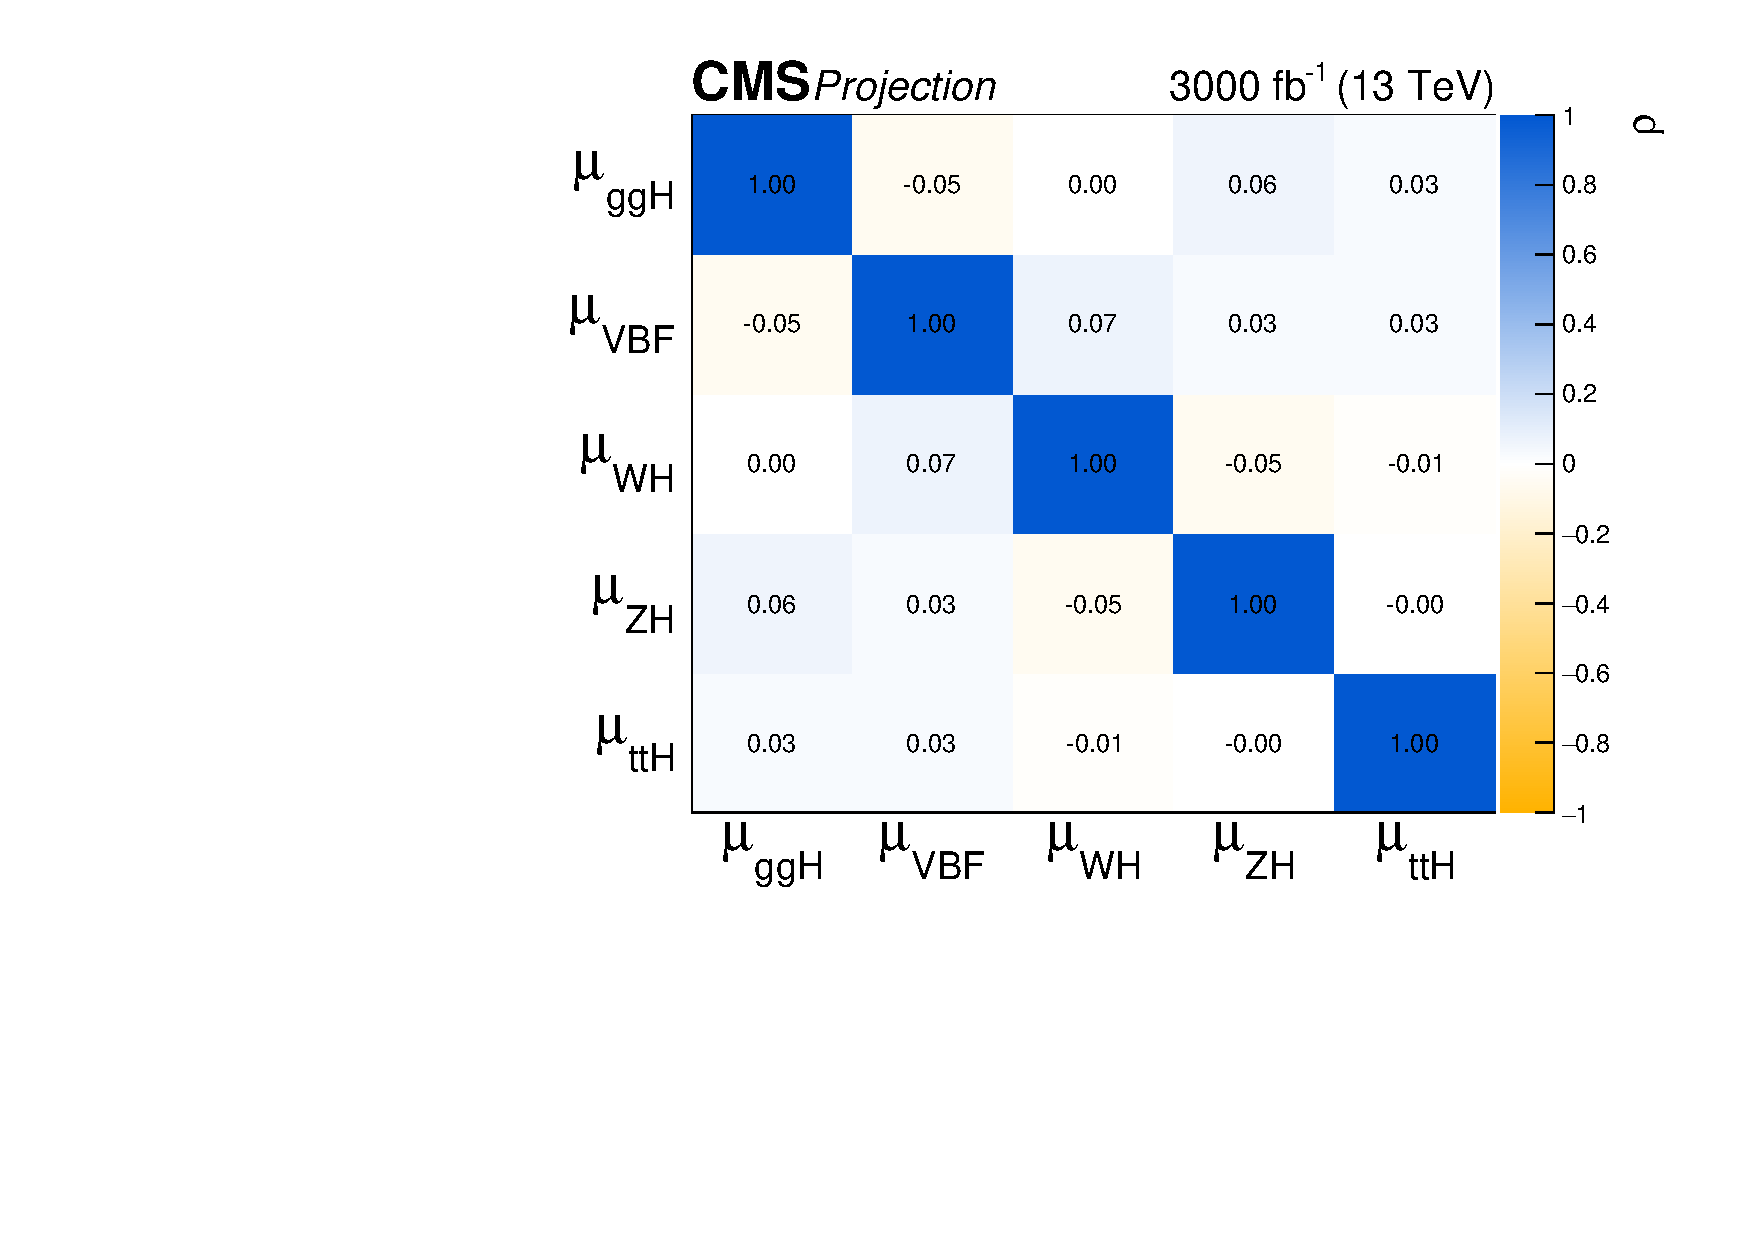
\includegraphics[width=0.48\textwidth]{\main/section2/plots/comb/correlations_A1_5P_S2_3000.pdf}%
\caption{Summary plot showing the total expected $\pm 1\sigma$ uncertainties in S2  (with YR18 systematic uncertainties) on the Higgs boson production mode cross-sections in different decay channels normalized to the SM predictions combining  ATLAS and CMS.}
\label{fig:comb_5PD}
\end{figure}
